\section{Introduction}

Modern web-based applications are implemented as multiple
agents simultaneously serving users, that work on shared data
objects replicated across geographically distributed machines. 
Historically, replication transparency (i.e. requiring distributed
systems to \emph{appear} as a single server and database to the users), has been viewd as the most
important proprty of such systems, which is resulted in extensive
studies around the implementation and reasoning techniques of {\bf
strongly consistent} distributed stores. Although the strong notions of
consistency, such as {\bf linearizability} and {\bf serializability}, 
are ideal for developing and reasoning about distributed applications, they
come with the price of availability and low response-time. 
%which are intrinsically crucial for web-based large-scale applications. 
To liberate the application instances from the extensive
synchronization required in strong consistency models and allows 
them to be "always-on" despite of unavoidable
network partitionings, {\bf weak consistency} models are taken into
account and distributed applications are instead designed to
tolerate certain inconsistencies. For example, user's $\mathtt{read}$ requests can
be immediately responded with the \emph{local state} of a server, if the users
can tolerate reading values that are not necessarily the latest ones.

Even though weak models of consistency (e.g. session guarantees from
Terry et. al.) have been known for more than two decades, they suffer 
from the lack of standardized definitions and enforcement
methodologies, which forces developers to modify their applications
with ad-hoc fixes in order to enforce their desired levels of
consistency. The lack of a
general reasoning framework for weak consistency models, has resulted in the
difficulty of proving correctness and optimality properties of such
highly error-prone implementations. To make the matter worse, many of
distributed applications require different \emph{combinations} of known
consistency guarantees, or might even face new consistency requirements
after the developement phase is over.

As an example, let's consider a distributed bulletin board application where users
send requests to a cloud of servers to post a message or to read the current
messages on the board. Each user request is sent to an available server,
which itself is working on top of an instance of an off-the-shelf data
store (e.g. Facebook's Cassandra). 
Since the underlying stores, usually satisfy the {\bf eventual consistency} model, 
developers are guaranteed  that every write to a local instance of the data 
store will eventually  be delivered at all other instances. However, 
most of the desirable application-level properties are not met under this model.          
For example, assume the developers wants to make sure that all the
$\mathtt{read}$ requests from
a user, would necessarily include prior writes by the same user.  This
guarantee which is known as {\bf read my writes (RMW)} can be violated in
eventually consistent stores.  
Here, delopers are forced to come up with their own implementation of
RMW. They must modify client and server applications to generate, send
and receive special tokens, to maintain the set of updates available at
each server, and block user requests, if some necessary updates are
still missing.


\begin{figure}[h]
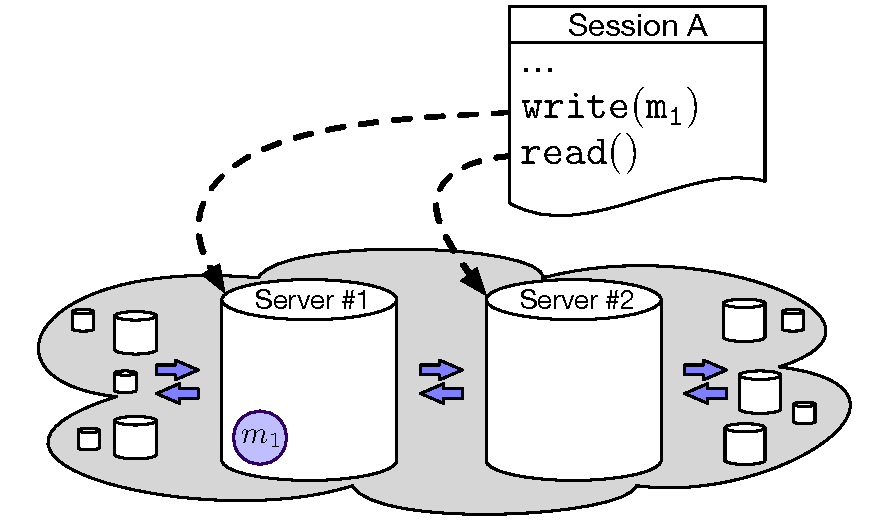
\includegraphics[scale=0.48]{../Figures/System_example.pdf}
\caption{A simple way of showing contracts}
\label{fig:ctrt}
\end{figure}



In this paper, we address these issues by introducing a principled approach to 
derive enforcement mechanisms for various forms of weak consistency 
guarantees. We offer developers with a language to specify their application-level consistency 
requirements as logical formulae expressing allowed relationships between update effects. 
We also introduce a new tool that generates a shim layer on top of the eventually 
consistent data store, and extends it to a key-value store with multiple environments, each of which 
shows the desired behavior specified by the given specifications. Our consistency enforcement 
methodology is independent of the underlying store, and only assumes the well established 
guarantee of "eventual delivery". 
Moreover, our specification language is also powerful enough to express all the known consistency 
guarantees in the context. 

We argue that all the consistency guarantees basically specify, \emph{when} an 
application instance should block a user request and for arrival of 
\emph{what} remote updates it should wait. For obvious reasons, any implementation of these 
consistency guarantees must be \emph{correct} and \emph{optimal}. The former property states that 
all possible behaviors of the implementation are allowed by the given specification and the later 
ensures that application instances do not engage in 
any unnecessary synchronization before responding to a user request (i.e. users are only blocked if 
it is absolutely necessary).
\\ Our technique is based on tracking relationships between update effects, and maintaining multiple 
(logical) caches at the shim layer, each of which is enforced to satisfy a specific level of consistency, 
derived from the given specifications. We believe that our approach is the first ever principled 
reasoning and implementation framework for weak consistency enforcement techniques which 
is also proven to be \emph{correct} and \emph{optimal}. 
By separating all the consistency management procedures from the application level, we are taking 
the non-trivial task of proving soundness criteria for ad-hoc consistency enforcement techniques 
off of the developer's shoulders. 
% Contributions of the paper
\\The paper makes the following contributions:
\begin{itemize}
\item Introducing a new specification language that covers all the known consistency guarantees in 
the context. Our language is arguably simpler than the previous works, and is based on observing 
similarities of different consistency requirements.

\item Proposing a principled consistency enforcement methodology that is 
complete for our specification language and allows deriving multi-purpose consistency enforcement 
tools.

\item Presenting proofs of correctness and optimality of our consistency enforcement methodology 
and introducing the first ever general reasoning framework for weak consistency guarantees. 

\item Introducing our tool called  \tool that realizes our consistency enforcement methods and 
extends an off-the-shelf eventually consistent data store (Cassandra) to a multi purpose key-value 
data store with the ability to guarantee any requested consistency level defined by the 
developers. 

\item Presenting the evaluation results showing the utility of \tool compared to a hard-coded
implementation of a weak consistency guarantee. 
\end{itemize}

% Structure of the paper
The rest of the paper is structured as follows. 
In section 2 we introduce the running example and explain problems associated with it. 
Section 3 introduces our system model, including the distributed underlying database model, our 
multi-purpose shim layer, and the formal definition of our specification language.
In section 4, we introduce our consistency enforcement strategy in detail and introduce the 
formal semantics of the shim layer. In section 5, we present the formal definitions 
and proofs of correctness of optimality properties of our shim. Sections 6 introduces our tool 
including 
the implementation details,  
which is followed by section 7, where the test results from running \tool on 
distributed real world machines are presented. 
We discuss the related works and future directions in the section 8. 
